\documentclass[a4paper]{article}

\usepackage{graphicx}          % For including graphics.
\usepackage{amsmath}           % Some mathematical symbols.

\addtolength{\topmargin}{-20mm}% Margin adjustments.
\addtolength{\textheight}{20mm}% Margin adjustments.

\begin{document}

\title{Image Enhancement Report\\
\large{EQ2330 Image and Video Processing, Project 1}}
\author{Harald Nordgren\\ haraldnordgren@gmail.com}
% \date{March 17, 2009} % Manual date

\maketitle

\section*{Summary}
\label{sec:summary}

I have investigated spatial and frequency domain image enhancement techniques in Matlab on the 512x512 demo image "Lena".

%Write a short summary of your report. Write approximately 150 words about the
%problem that you are considering, your solution, obtained results and the
%the conclusion. For example, this template provides instructions for writing the
%project reports for the EQ2330 Image Processing course. Read it thoroughly as it
%is expected that the instructions are followed.

\section{Introduction}
\label{sec:introduction}

This project was about restoring images the were degraded using three types of techniques.

The first sub-assigment deals with the dynamic range of greyscale images where intensity values are found in the range [0,255]. Looping over each pixel value and summing the pixel values into bins (one bin for all intensity values 0, one for 1, and so on) creates a histogram. A normal-looking image will have a histogram that uses the whole dynamic range and spreads somewhat evenly.

Using the function

\begin{equation}
	\label{dr}
	g(x, y) = min(max(\left\lfloor 0.2 \cdot  f (x, y) + 50 \right \rceil, 0), 255)
\end{equation}

the dynamic range can be lowered but squeezing the values together, giving a duller-looking image. Assuming an image that for some reason starts out with a small dynamic range, histogram equalization can stretch the dynamic range to the entire 8-bit spectrum, giving a more lively apperance. The cumulative sum of the normalized histogram for the low-contrast image can be calculated as follows

\begin{equation}
	s_k = 255 \sum_{j=0}^{k} p_r(r_j)
\end{equation}

where the dynamic range the dynamic range is stretched to [0,255]. p is the probability for each intensity value in the original image, and the sum for p over the entire numerical axis is 1 by definition. Mapping the intensity values of the low-contrast image to these summed values equalizes its histogram.

In the second sub-assignment, the \texttt{mynoisegen} function generates two types of noise that are applied to the original images, and I then attempt to recover it. The Gaussian noise is additive, after which I requnatize the image to bring it back to the [0,255] interval. The salt-and-pepper noise sets certain random pixel values to 0 or 255, which represent black and white, respectively giving the impression that the image has been salted and peppered.

The attempts to recover the noised image realy of two very similar methods. The mean filter uses a kernel of a certain size (here a 3x3 matrix with every value equal to 1/9) which is convoluted with the noised image, effectively averaging each pixel value with its closest neighbors. The median filter replaces each pixel with the median of the neighboring pixels, meaning that these values have to be sorted first. Both methods remove high-frequency noise alongside legitimate information from the image.

In the final sub-assignment, the image is blurred by convoluting with a Gauss kernel generated by \texttt{myblurgen} and then quantized to give additive noise, modeled as

\begin{equation}
	f(x,y) = g(x,y) * h(x,y) + \eta(x,y)
\end{equation}

The task is then to deblur the image while only using the blurring function and the variance of the noise.

%Give an introduction to the problem considered. The introduction should be
%written such that it can be understood by an engineer whose area of expertise is
%not image processing. Motivate the problem by using references to work by other
%authors~\cite{coursebook}, as well as interesting applications.

%Define the mathematical notation used in the report and state the problem using
%this notation. Make sure that any assumptions you are using are explicit. It is
%often convenient to be able to refer to equations by numbers. An example
%equation is the additive noise degradation model for images

%\begin{equation}
%  \label{eqn:model}
%  g(x,y) = f(x,y) + \eta(x,y).
%\end{equation}

\section{System Description}
\label{sec:system}
In the first sub-assignment, I plotted the histogram for the three versions of the demo image, using \texttt{subplot}. To calculate histograms all matrices are first converted to an array vector with \texttt{(:)} and divided each value by the total sum before plotting as a bar graph.

To lower the contrast I iterated over each pixel and calculate \eqref{dr}, and to equalize the histogram I used \texttt{cumsum} and then mapped the low-contrast values to the summed function.

I used mynoisegen to add Gaussian and Salt-and-pepper noise to the original, and then tried removing it with mean and median filtering. The mean filter replaces each value with the mean of the surrounding values. The median replaces it with the median (that is, sorting the values by size and choosing the middle one). The mean filter is quicker to calculate -- no sorting is needed -- but the median filter is likely to give slightly better results when dealing with outlier noise, which is why it gives such a good performance for the salt-and-pepper noise.

In the last task, I applied Gaussian blur by convolution the original images with a 8x8 kernel generated by myblurgen, and quantized the this image to 8-bit -- giving additive noise. Given the symmetry of the blur kernel (leading to a zero determinant) it is obvious that a simple inverse filter would not do. Using the variance of the quantization noise and the blurring function, I used \texttt{deconvwnr} to deblur the image.

To avoid ringings along the border of the image, I had to first run \texttt{edgetaper}. I then plotted original, degenerated and deblurred images, along with their fourier spectra.

\section{Results}
\label{sec:results}

The histogram for the low-contrast image looks like what you would expect, squeezed togther, but still maintaining the overall shape. The low-contrast image seems looks like it's hidden behind a screen and could be brought out by the correct means. The equalized image looks great, maybe even better than the original, although the light areas are maybe too light, and edges, like the hat and its feather look "over-sharp".

For a continuous probability density function we expect equalization to give a completely flat histogram, but for out quantized data it will show slight deviations from that but will be as close as possible.

\begin{figure}[!ht]
  \centering
  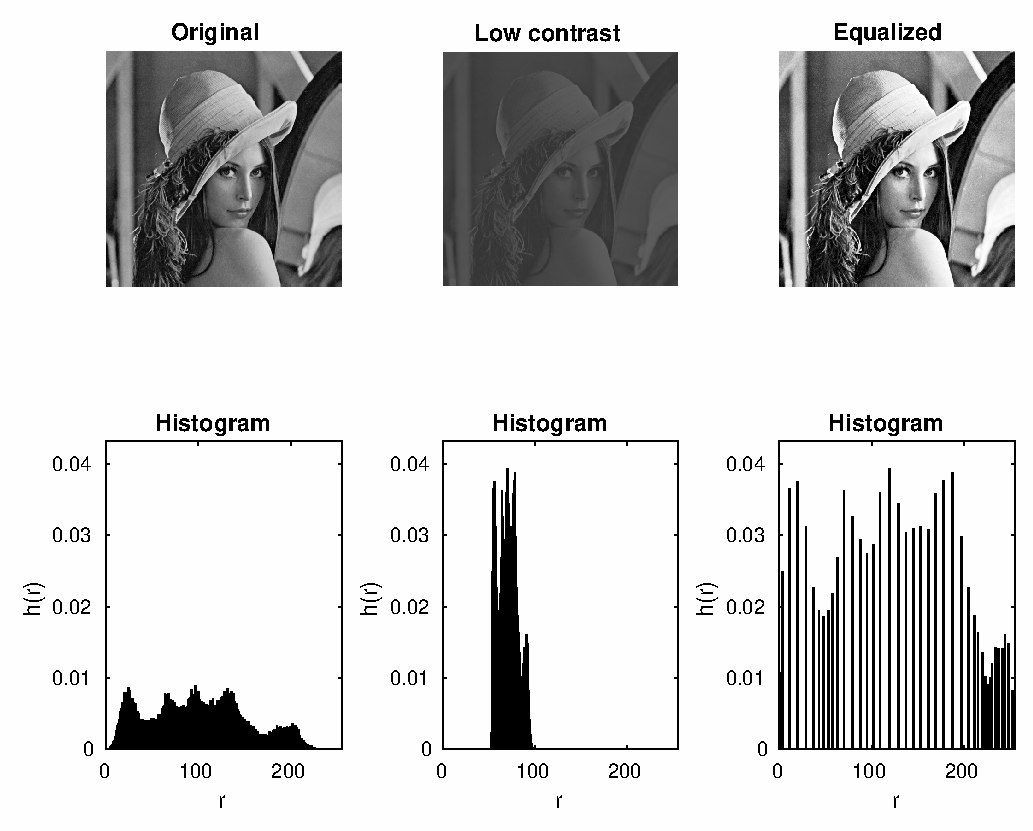
\includegraphics[width=0.9\columnwidth]{images/2-1.eps}
  \caption{Sub-assigment 2.1}
  \label{fig:21}
\end{figure}

\begin{figure}[!ht]
  \centering
  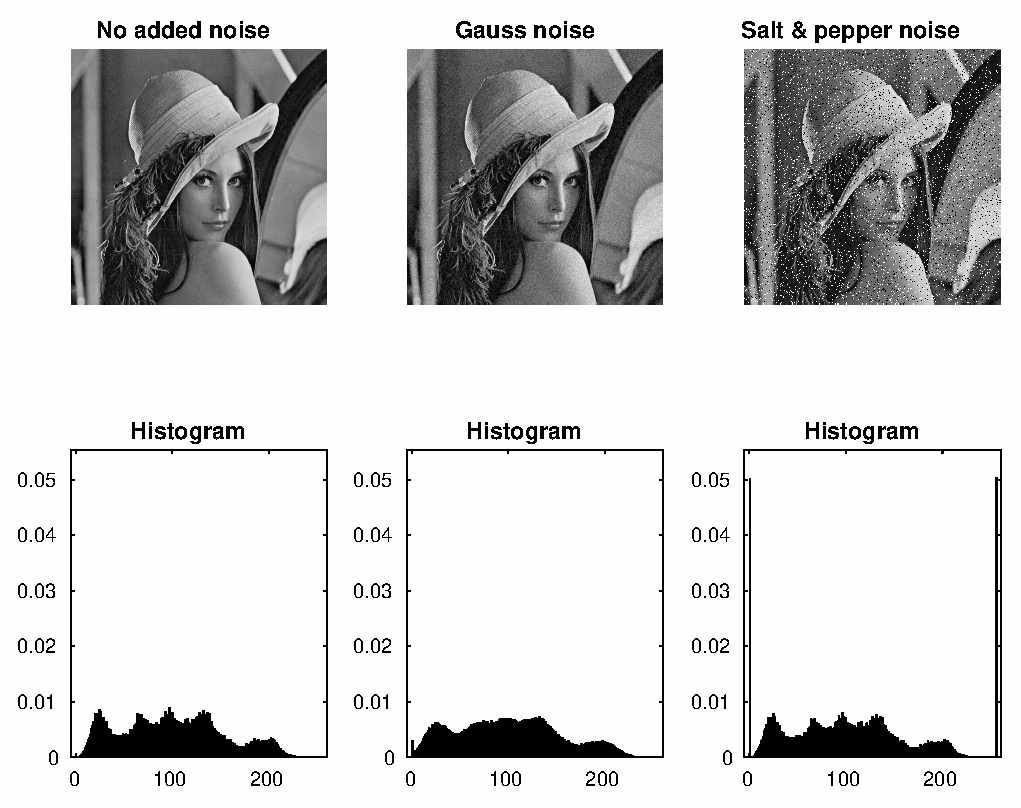
\includegraphics[width=0.9\columnwidth]{images/2-2_noised.eps}
  \caption{Sub-assigment 2.2 Noised added}
  \label{fig:22n}
\end{figure}

\begin{figure}[!ht]
  \centering
  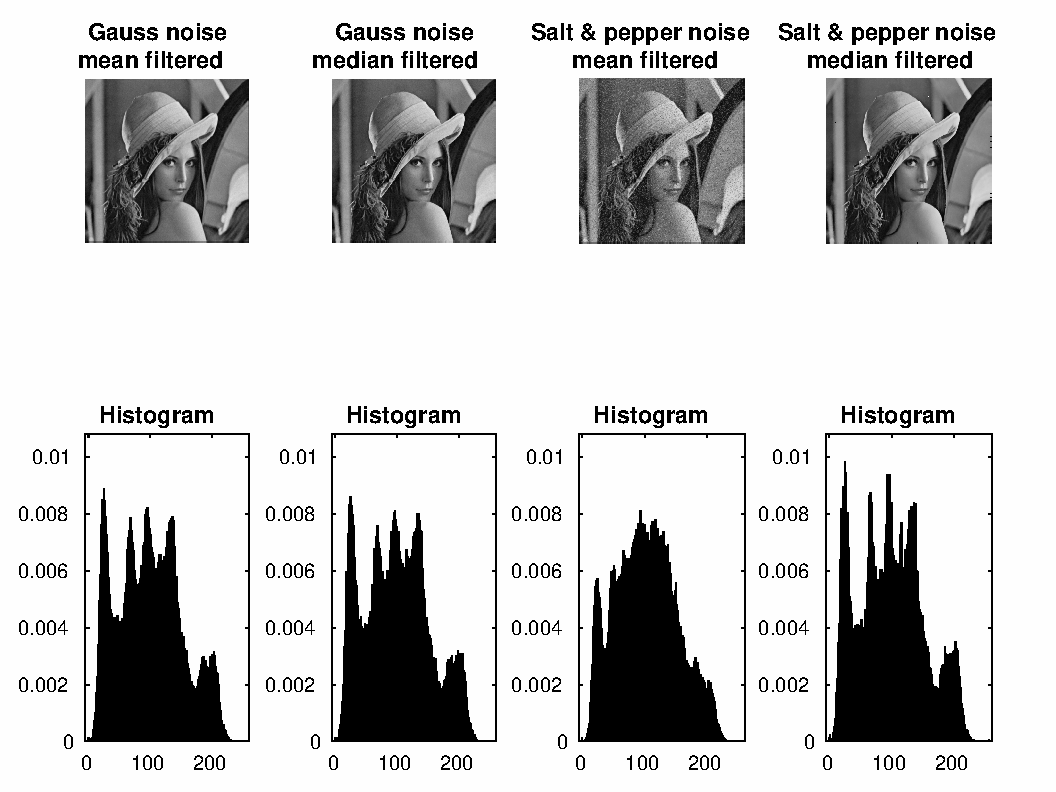
\includegraphics[width=0.9\columnwidth]{images/2-2_filtered.eps}
  \caption{Sub-assigment 2.2 Filtered}
  \label{fig:22f}
\end{figure}

\begin{figure}[!ht]
  \centering
  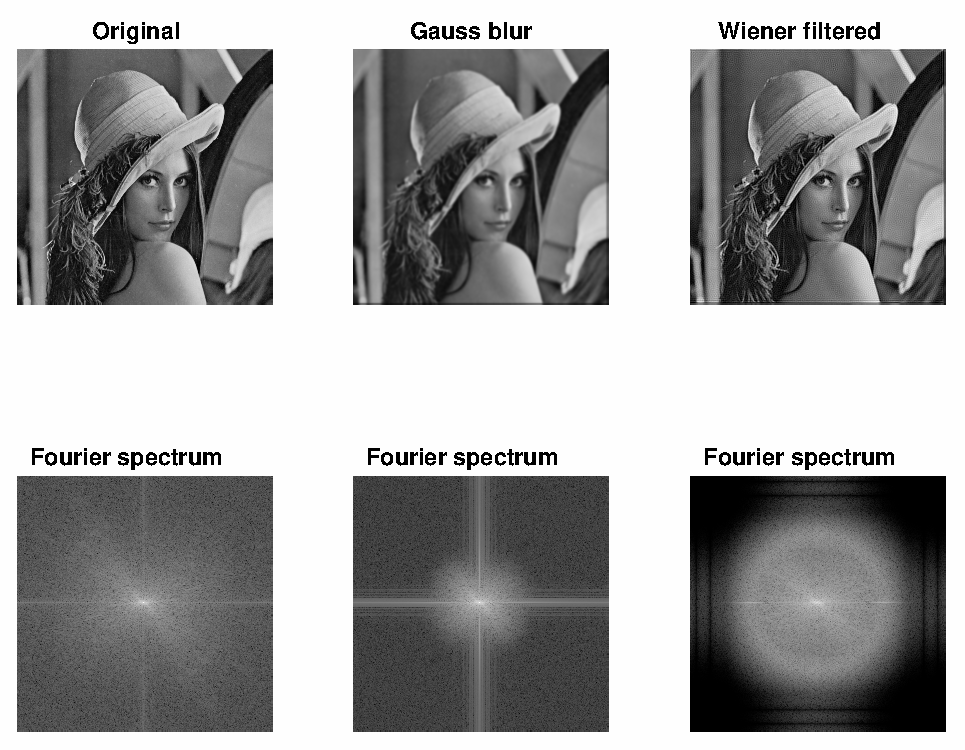
\includegraphics[width=0.9\columnwidth]{images/3.eps}
  \caption{Sub-assigment 3}
  \label{fig:3}
\end{figure}

\section{Conclusions}
\label{sec:conclusions}

Present your conclusions in this section. Remember that conclusions are not just
another summary. Your report, excluding references and appendix, should fit in
4-5 A4-pages. Therefore, make sure to write concisely and to the point,
describing everything of importance. Writing a report takes time, which is why
you should start early. If you have any questions about the assignment ask the
teaching assistants in time. Name your report pdf-file in the format
\verb\20YYpX_author1_author2.pdf\, where \verb\author1\ and \verb\author2\ are
surnames of the authors.

\section*{Appendix}

\subsection*{Who Did What}
Describe in detail how the project work was divided between the authors.
This template was written by Ermin Kozica in \LaTeXe. A good introduction to
\LaTeXe is available at~\cite{latexmanual}. You can write your report in other
programs as well.

\subsection*{MatLab code}
Include the well documented MatLab code that you have used.
\begin{verbatim}
function h = histogram(f)
% A function that calculates the histogram of matrix f.

N = numel(f); % The number of elements in f
h = ...
\end{verbatim}


\begin{thebibliography}{99}
\bibitem{coursebook} Rafael C. Gonzalez and Richard E. Woods,
  \textsl{Digital Image Processing},
  Prentice Hall, 2nd ed., 2002
\bibitem{latexmanual} Tobias Oetiker et al.,
  \textsl{The Not So Short Introduction to \LaTeXe},
  Available: http://tobi.oetiker.ch/lshort/lshort.pdf,
  Last accessed: March 17, 2009
\end{thebibliography}
\end{document}
